\documentclass{scrartcl}
\usepackage[utf8]{inputenc} 
\usepackage[T1]{fontenc}
\usepackage{lmodern}
\usepackage[ngerman]{babel}
\usepackage{courier}
\usepackage{amsmath}
\usepackage{graphicx}
\usepackage{multicol}
\usepackage{geometry}
\usepackage{authblk}
\usepackage[font=scriptsize, labelfont=bf]{caption}
\newenvironment{Figure}
  {\par\medskip\noindent\minipage{\linewidth}}
  {\endminipage\par\medskip}


% for skript letters like H...
\usepackage{mathrsfs}

\geometry{verbose,a4paper,tmargin=25mm,bmargin=25mm,lmargin=15mm,rmargin=20mm}

\title{Protokoll zum Versuch Nichtlineare Dynamik und Chaos}
\author{Nicolas Heimann, Jesse Hinrichsen}
\affil{\textit{Universität Hamburg}}
\date{2015}
\begin{document}
\maketitle




\begin{description}
\item Zusammenfassung
\end{description}


\section{  Einleitung  }
LALALA

\section{Logistische Abbildung}
$$x_{n+1}=f_r(x_n)=rx_n(1-x_n)$$
Def.: $f^2(x) = f(f(x))$
$$\Rightarrow x_{n+2}=r^2x_n(1-x_n)(1-rx_n(1-x_n))$$
\newline
Fixpunktgleichung (Einerzyklus): 
$$x=rx(1-x)$$
$$\Rightarrow x_1=0, x_2=1-\frac{1}{r}$$
Startwerte x=0 und x=1 haben den Fixpunkt $x_1$ wohingegen für alle $x\in (0,1)$ der Fixpunkt $x_2$ ist.
\newline
Fixpunktgleichung (Zweierzyklus):
$$x=r^2x(1-x)(1-rx(1-x))$$
$$\Rightarrow x_{3,4}=\pm\frac{\sqrt{r^2-2 r-3}+r+1}{2 r}$$
Damit $x_{3,4}$ reel bleibt muss $r^2-2 r-3 \geq 0$
$$\Rightarrow r \leq -1 \land r \geq 3$$
Für diesen Bereich gibt es folglich 2 weitere Fixpunkte $x_{3,4} \Leftrightarrow$ Perdiodenverdopplung 
\newline
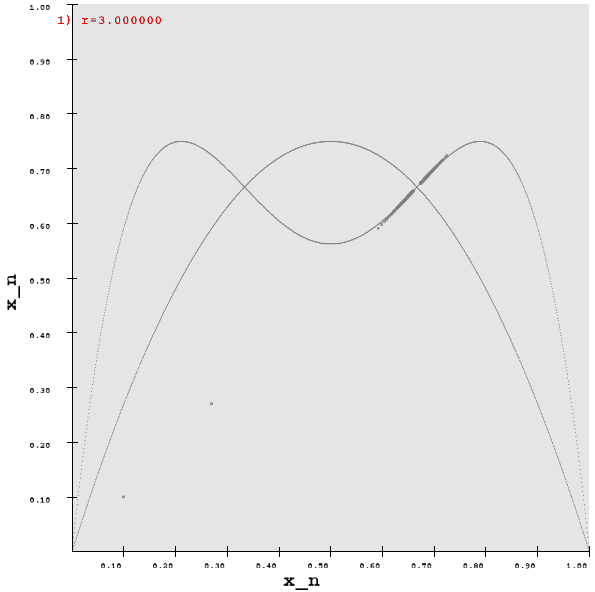
\includegraphics[scale=0.3]{r3}
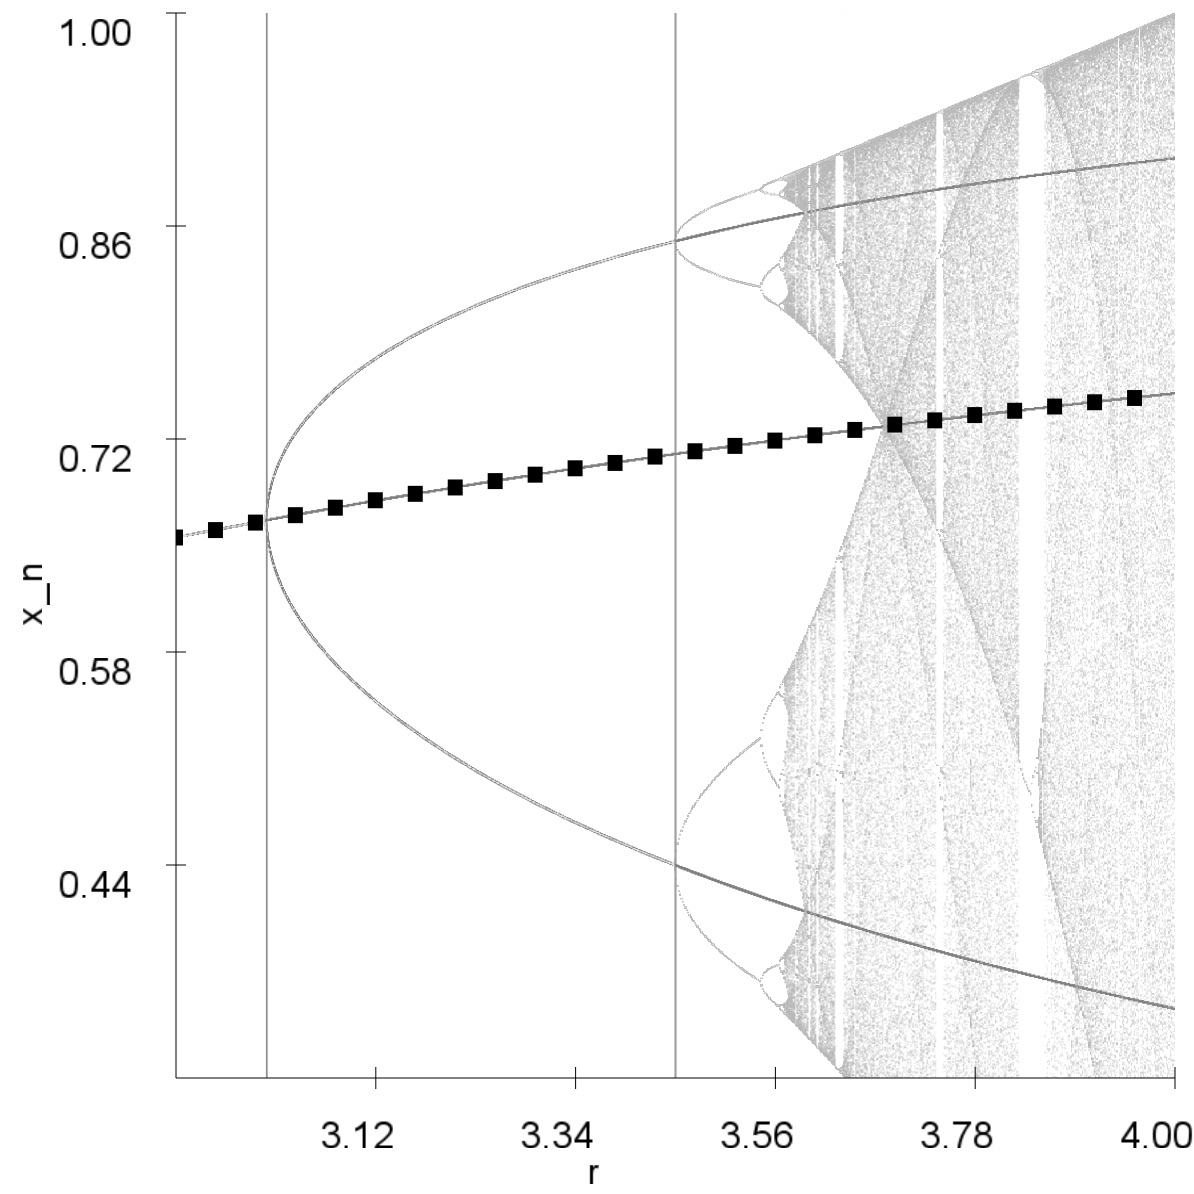
\includegraphics[scale=0.3]{analy-periodenv}
\newline
\subsection{ Stabilitätsbedingung }
Ein Fixpunkt ist stabil, wenn gilt:
$$\mid f'(x)\mid <1$$
Im Fall der logistischen Abbildung gilt
$$\frac{d}{dx}f(x)=r-2rx=r(1-2x)$$
$$\frac{d}{dx}f^2(x)=-r^2(2x-1)(2r(x-1)x+1)$$
\newline
Es gilt zu lösen, für welche $r$ bei bekannten Fixpunkte die Stabilitätsbedingung erfüllt ist.
\newline
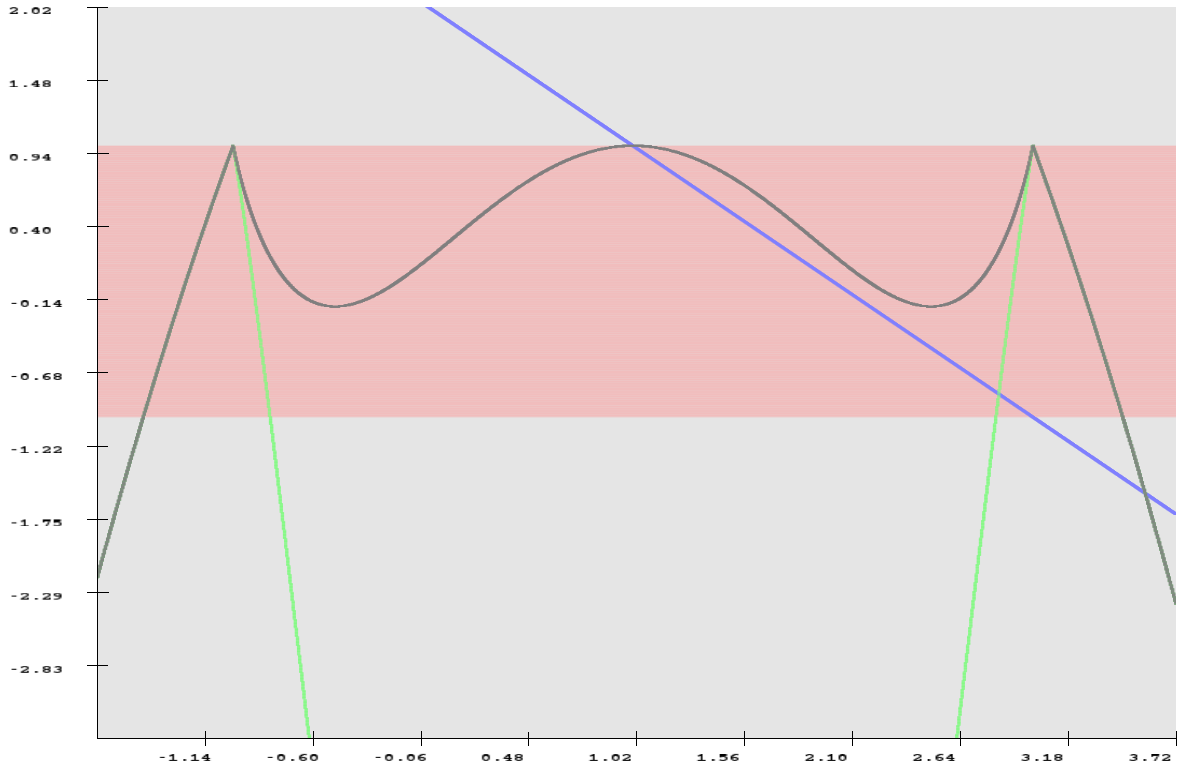
\includegraphics[scale=0.4]{stable_fixpoints}
\newline
Grafisch lässt sich ablesen, dass der Fixpunkt $x_3=\frac{\sqrt{r^2-2 r-3}+r+1}{2 r}$ (grüner Graph) für folgende Bereiche stabil ist:
$$-1.45<r<-0.82 \Rightarrow -1.45 < r \leq -1$$
$$2.82<r<3.45 \Rightarrow 3 \geq r > 3.45$$
Der Fixpunkt $x_4=\frac{-\sqrt{r^2-2 r-3}+r+1}{2 r}$ (grauer Graph) ist im gesamten Bereich $-1.45<r<3.45$ stabil aber da der Fixpunkt ebenfalls nur für $r \leq -1 \land r \geq 3$ existiert gilt der selbe Bereich wie für $x_3$. Die Fixpunkt sind dort stabil, wo sich der graue und der grüne Graph in der Abbildung überlagern.
\section{ Feigenbaumkonstante}
\subsection {Lyapunov}
Eine Möglichkeit die Feigenbaumkonstante zu berechnen ist über die Nullstellen des Lyapunov-Exponenten. Gerade an diesen Stellen kommt es zu einer Periodenverdopplung.

\section{ Literatur }
\begin{itemize} 
\item Nichtlineare Dynamik und Chaos - Physikalisches Praktikum für Fortgeschrittene Universität Hamburg
\end{itemize}




\end{document}







